\documentclass[20pt, a1paper, portrait, margin=0mm, innermargin=10mm,
     blockverticalspace=10mm, colspace=10mm, subcolspace=8mm]{tikzposter}

\usepackage{amssymb,amsmath}
\usepackage{mathtools}
\usepackage{ntheorem}

\usepackage{graphicx}
\usepackage{xcolor}
\usepackage{adjustbox}
\usepackage{tikz}
\usetikzlibrary{automata,arrows,positioning}

% Orange brand colours
% core colours
\definecolor{brand-orange}{RGB}{255,121,0}
% support colours
\definecolor{brand-blue}{RGB}{75,180,230}
% functional greys
\definecolor{brand-lightgrey}{RGB}{246,246,246}
% functional colours
\definecolor{brand-func-blue}{RGB}{82,126,219}

\tikzstyle{switch-style}=[circle, draw, thin, fill=brand-func-blue, scale=0.3]
\tikzstyle{controller-style}=[rectangle, thin, fill=brand-orange, scale=0.8]
\tikzstyle{rpath}=[ultra thick, brand-orange, opacity=0.4]
\tikzstyle{punkt}=[rectangle, rounded corners, draw=black, very thick, minimum height=2em, text centered]

\theoremstyle{break}
\newtheorem*{theorem}{Theorem}

\title{Epidemic Control with Learning \& Optimization}
\author{Cristina Bazgan$^{\dagger}$, Paul Beaujean$^{\dagger *}$, \'Eric
	Gourdin$^{*}$}
\institute{$^{\dagger}$LAMSADE, Universit\'e Paris-Dauphine, $^{*}$Orange Labs}
\titlegraphic{
}

\makeatletter
\renewcommand\TP@maketitle{%
   \centering
   \begin{minipage}[b]{0.8\linewidth}
        \centering
        \color{titlefgcolor}
        {\bfseries \Huge \sc \@title \par}
        \vspace*{1em}
        {\huge \@author \par}
        \vspace*{1em}
        {\LARGE \@institute}
    \end{minipage}%
    \tikz[remember picture, overlay]
    \node[scale=0.8,anchor=east,xshift=0.56\linewidth,yshift=3cm,inner sep=0pt] {
	\includegraphics[width=0.1\textwidth]{logo_cmyk}
    };
    \tikz[remember picture, overlay]
    \node[scale=0.8,anchor=east,xshift=-0.6\linewidth,yshift=2cm,inner sep=0pt] {%
	\includegraphics[width=0.1\textwidth]{dauphine-logo}
    };
}
\makeatother

% Choose LAYOUT:  Default, Basic, Rays, Simple, Envelope, Wave, Board, Autumn, Desert,
\usetheme{Autumn}
\usecolorstyle[colorOne=brand-func-blue, colorTwo=brand-lightgrey,
colorThree=brand-func-blue]{Germany}

\begin{document}
\maketitle{}

\begin{columns}
  \column{0.4}
  \block{Context}{
    \begin{itemize}
      \item[$\circ$] Software-defined networking enables full automated control
	over network topology.
      \item[$\circ$] Networked systems face propagation of malware, cascading
	hardware failures, DDoS.
    \end{itemize}
    \begin{tikzfigure}[SDN Controller supervising a software-defined network]
      \begin{tikzpicture}[auto, thick]
       % Cloud creation
       \node[cloud, fill=brand-lightgrey, cloud puffs=16, cloud puff arc= 100,
	minimum width=7cm, minimum height=2.5cm, aspect=1] (cloud) at (0,0) {};
	\node (cloud-legend)[right=0.5cm of cloud] {Logical Topology};

       % Physical layer nodes
	\foreach \place/\x in {{(-2.5,0.3)/1}, {(-1.75,-0.55)/2},{(-1.2,0.55)/3},
	  {(-0.75,-0.7)/4}, {(-0.25,0)/5}, {(0.25,0.7)/6}, {(0.75,-0.3)/7},
	  {(1.5,0)/8},{(2.5,0.4)/9}}
	\node[switch-style] (a\x) at \place {};

	% SDN topology links
	\path[thin] (a1) edge (a2);
	\path[thin] (a1) edge (a3);
	\path[thin] (a2) edge (a3);
	\path[thin] (a3) edge (a6);
	\path[thin] (a2) edge (a4);
	\path[thin] (a5) edge (a6);
	\path[thin] (a5) edge (a4);
	\path[thin] (a5) edge (a2);
	\path[thin] (a5) edge (a7);
	\path[thin] (a6) edge (a7);
	\path[thin] (a6) edge (a9);
	\path[thin] (a6) edge (a8);
	\path[thin] (a8) edge (a9);
	\path[thin] (a7) edge (a8);
 
	\node[controller-style] (b)[above=3cm of a5] {};
	\node (b-legend)[right=1cm of b] {SDN Controller};
 
	\foreach \i in {1,...,9} \path[rpath] (a\i) edge (b);

      \end{tikzpicture}
  \end{tikzfigure}
  }

  \column{0.6}
  \block{Model}{
    \begin{minipage}[t]{0.25\textwidth}
      \begin{itemize}
	\item[$\circ$] Epidemics spreading on undirected graphs.
	\item[$\circ$] Markov process with transition rates depending on
	  neighbour state.
	\item[$\circ$] Epidemics spreading on undirected graphs.
      \end{itemize}
    \end{minipage}
    \begin{minipage}[t]{0.35\textwidth}
      \begin{tikzfigure}[$\text{SIS}(\beta,\delta)$ of a node $v$]
	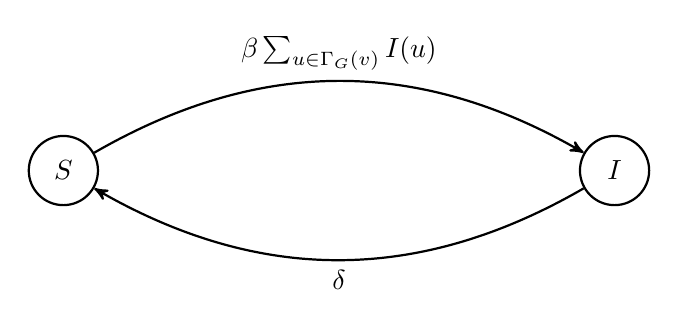
\begin{tikzpicture}[->, >=stealth', auto, thick, node distance=7cm]
	\tikzstyle{every state}=[fill=white, draw=black, thick, text=black, scale=1]

	\node[state] (S) {$S$};
	\node[state] (I)[right of=S] {$I$};

	\path (S) edge [bend left] node[above] {$\beta \sum_{u \in \Gamma_G(v)} I(u)$} (I);
	\path (I) edge [bend left] node[below] {$\delta$} (S);

	\end{tikzpicture}
      \end{tikzfigure}
    \end{minipage}
  }
\end{columns}

\block{General framework}{

  \begin{minipage}[t]{0.5\textwidth}
    \begin{tikzfigure}[Control loop]
      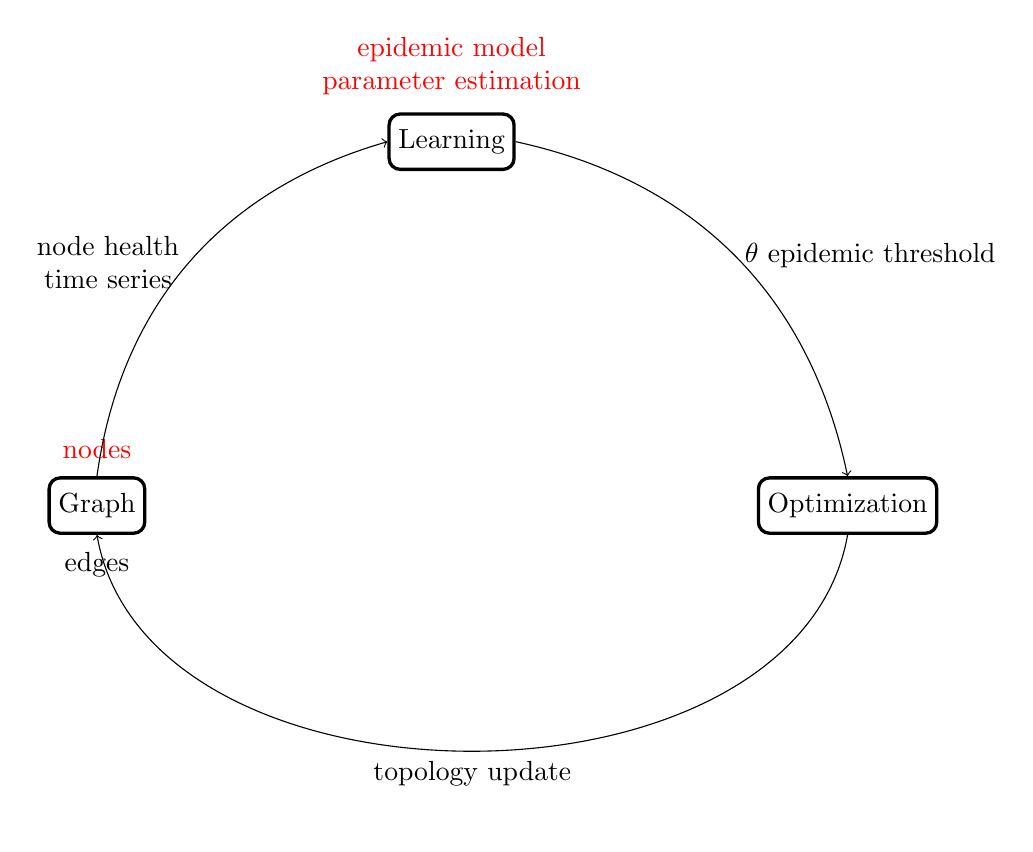
\begin{tikzpicture}[auto, node distance=4cm]
      
	\node (control) {};

	\node[punkt] (graph) [left=of control.south east] {Graph};
	\node[above=0.1cm of graph, text=red] {nodes};
	\node[below=0.1cm of graph] {edges};

	\node[punkt] (optimization) [right=of control.south west]  {Optimization};
	
	\node[punkt] (learning) [above=of control.north] {Learning};
	\node[above=0.1cm of learning, text=red, align=center] {epidemic model\\parameter estimation};

	\path (graph.north) edge [->, bend left=33, align=center] node[left] {node health\\time series}
		(learning.west);
	\path (learning.east) edge [->, bend left=33, align=center]
	node[right] {$\theta$ epidemic threshold} (optimization.north);
	\path (optimization.south) edge [->, bend left=80] node[below] {topology update}
		(graph.south);
      \end{tikzpicture}
    \end{tikzfigure}
  \end{minipage}
  \begin{adjustbox}{valign=t}
      \begin{minipage}[t]{0.4\textwidth}

	\subsection*{Turning a theorem into a control system}
	\begin{theorem}[Ganesh et al., 2005]
	  For any propagation model of threshold $\theta$ on a graph
	  $G$, the epidemic dies out in logarithmic time if
	  \begin{equation*}
	    \lambda_{\max}(G) < \theta.
	  \end{equation*}
	\end{theorem}

	Instead of applying local security measures, we leverage the control on
	the software-defined network topology to extinguish a propagating
	threat.
	
	\subsection*{}
      
      \end{minipage}
  \end{adjustbox}
}

\block{Learning the epidemic threshold}{

    \begin{minipage}[t]{0.6\textwidth}
      \begin{tikzfigure}[One Class SVM for Anomaly Detection]
      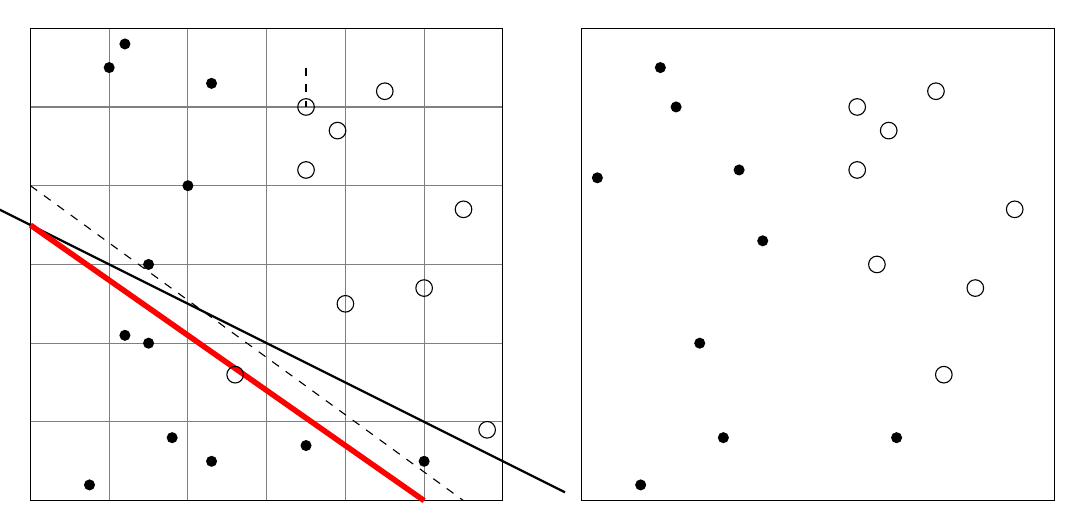
\begin{tikzpicture}
	\draw[color=gray] (0,0) grid (6,6);
	\draw (0,0) rectangle (6,6);

	\coordinate (SV1) at (1,3);
	\coordinate (SV2) at (5,1);

	\draw [black, thick, shorten >= -2cm, shorten <= -2cm] (SV1)--(SV2);

	% \draw line
	\draw[color=red,line width=2pt] (0,3.5) -- (5,0);
	% \draw dashed line
	\draw[dashed]  (0,4) -- (5.5,0);
	\draw[dashed]  (3.5,5.5) -- (3.5,5);

	\draw (7,0) rectangle (13,6);
	  
	\def\positive{{%
	{2.3,5.3},
	{3.5,.7},
	{1.5,2},
	{1.2,2.1},
	{1.8,.8},
	{1,5.5},
	{1.2,5.8},
	{.75,.2},
	{2,4},
	{5, 0.5},
	{1.5,3},
	{2.3,.5},
	%
	{9.3,3.3},
	{11,.8},
	{8.5,2},
	{7.2,4.1},
	{8.8,.8},
	{8,5.5},
	{8.2,5},
	{7.75,.2},
	{9,4.2},
	{12, 0.5},
	{8.5,3},
	{9.3,.5},
	}}
	  
	% \draw positive dots
	\foreach \i in {0,...,20} {
	  \pgfmathparse{\positive[\i][0]}\let \x \pgfmathresult;
	  \pgfmathparse{\positive[\i][1]}\let \y \pgfmathresult;
	  \fill[black] (\x,\y) circle (2pt);
	}
	  
	\def\negative{{%
	{4,2.5},
	{3.5,5},
	{2.6,1.6},
	{4.5,5.2},
	{5.5,3.7},
	{3.9,4.7},
	{5,2.7},
	{3.5,4.2},
	{5.8,.9},
	%
	{10.75,3},
	{10.5,5},
	{11.6,1.6},
	{11.5,5.2},
	{12.5,3.7},
	{10.9,4.7},
	{12,2.7},
	{10.5,4.2},
	{12.8,.9},
	}}
	  
	% \draw negative dots
	\foreach \i in {0,...,16} {
	  \pgfmathparse{\negative[\i][0]}\let \x \pgfmathresult;
	  \pgfmathparse{\negative[\i][1]}\let \y \pgfmathresult;
	  \draw[black] (\x,\y) circle (3pt);
	}
	\end{tikzpicture}
    \end{tikzfigure}
  \end{minipage}
  \begin{adjustbox}{valign=t}
      \begin{minipage}[t]{0.3\textwidth}
	SDN Controller running a parameter estimation algorithm

	\begin{tikzfigure}[Closed walks of size $\log n$]
	    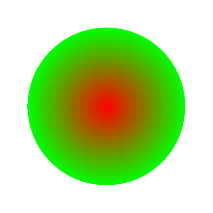
\begin{tikzpicture}
	      \draw[draw=none,inner color=red, outer color=green] (0,0) circle (1cm);
	    \end{tikzpicture}
	\end{tikzfigure}
      \end{minipage}
  \end{adjustbox}
}

\block{Optimizing the spectral radius}{

    \begin{minipage}[t]{0.3\textwidth}
    \begin{equation}
      \begin{split}
	\max & \sum_{e \in E} x_e\\
	  & A(x) \preceq t I\\
	  & x \in \{0,1\}^m
      \end{split}
    \end{equation}

  \end{minipage}
  \begin{adjustbox}{valign=t}
      \begin{minipage}[t]{0.7\textwidth}

	\innerblock{}{Combinatorics: subgraphs and closed walks
	}
	\innerblock{}{Random Matrix Theory: randomized algorithms relying on concentration of measure
	}
	\innerblock{}{Polynomials: real-stable polynomials and interlacing
	  families
	}
      \end{minipage}
  \end{adjustbox}
}

\end{document}
